\documentclass[aspectratio=169]{beamer}
\usetheme{Madrid}
\usecolortheme{default}
\usepackage{tikz}
\usetikzlibrary{calc}

% --- Organization slides (TOC + section dividers) ---
\AtBeginSection[]
{
  \begin{frame}{Outline}
    \tableofcontents[currentsection]
  \end{frame}
}

\title{Lecture 2: Marketing Automation with HITL}
\subtitle{Structured outputs, evaluation loops, and human review}
\author{University of Chicago}
\date{\today}

\begin{document}

\frame{\titlepage}

% Global outline (matches \section{} titles)
\begin{frame}{Outline}
  \tableofcontents
\end{frame}

\section{Development Methodology}

\begin{frame}{System Thinking: Breaking Down AI Tasks}
\begin{itemize}
    \item Before coding, we need to \textbf{think systematically}:
    \begin{enumerate}
        \item How do we abstract and organize our code?
        \item How do we break tasks into inputs and outputs?
        \item How do we organize these into functions?
    \end{enumerate}
    \item \textbf{Plan before you code}
    \item Break down required tasks, \textit{then} start coding
\end{itemize}
\end{frame}

\begin{frame}{Methodology: Vertical Slices}
\begin{itemize}
    \item AI systems are complex
    \item Rather than ``boiling the ocean,'' concentrate on \textbf{vertical slices}
    \item Build the \textbf{entire flow} that works \textit{in the simplest, single case}
    \item Then expand horizontally with more features
\end{itemize}
\vspace{0.5cm}
\textbf{Example}: CRM Email System
\begin{itemize}
    \item \textbf{Vertical slice}: One prospect $\rightarrow$ generate one email $\rightarrow$ verify output
    \item \textbf{Horizontal expansion}: Batch processing, error handling, A/B testing
\end{itemize}
\end{frame}

\begin{frame}{Methodology: Crawl, Walk, Run}
\begin{itemize}
    \item \textbf{Crawl}: What is the minimum code to verify it's possible?
    \begin{itemize}
        \item Hardcoded examples
        \item Manual verification
        \item Proof of concept that it can work in \textit{some} instances
    \end{itemize}
    \item \textbf{Walk}: What is the minimum code to verify it works in most cases?
    \begin{itemize}
        \item Handle common edge cases
        \item Basic error handling
        \item Works reliably for typical inputs
    \end{itemize}
    \item \textbf{Run}: What does the full production system look like?
    \begin{itemize}
        \item Comprehensive error handling
        \item Monitoring and logging
        \item Scale and performance optimization
    \end{itemize}
\end{itemize}
\end{frame}

\begin{frame}{Question: MVP vs. Crawl/Walk/Run}
\begin{center}
\Large
Is the MVP the ``Crawl'' or the ``Run''?
\end{center}
\vspace{1cm}
\pause
\textbf{Answer}: It depends on your definition of MVP
\begin{itemize}
    \item \textbf{Crawl} = Technical MVP (does it work at all?)
    \item \textbf{Walk} = Product MVP (can users use it reliably?)
    \item \textbf{Run} = Production system (can it scale?)
\end{itemize}
\end{frame}

\begin{frame}{Applying This Methodology}
In Lectures 2-4, we'll use this approach:
\begin{enumerate}
    \item \textbf{Crawl}: Build simplest working version
    \begin{itemize}
        \item Lecture 2: Generate one marketing email
        \item Lecture 3: Classify one support ticket
        \item Lecture 4: Research one topic
    \end{itemize}
    \item \textbf{Walk}: Add reliability and common cases
    \begin{itemize}
        \item Error handling
        \item Multiple examples
        \item User feedback
    \end{itemize}
    \item \textbf{Run}: Discuss production considerations
    \begin{itemize}
        \item Scale, monitoring, cost optimization
    \end{itemize}
\end{enumerate}
\end{frame}

\section{Building Modular AI Systems}

\begin{frame}{The Challenge: AI System Complexity}
\begin{itemize}
    \item AI systems involve many moving parts:
    \begin{itemize}
        \item Data preprocessing and validation
        \item Prompt engineering and model calls
        \item Response parsing and validation
        \item Error handling and retries
        \item Logging and monitoring
    \end{itemize}
    \item \textbf{Problem:} Trying to build everything at once leads to:
    \begin{itemize}
        \item Unclear failure points
        \item Difficult debugging
        \item Hard to test individual components
        \item Tight coupling between components
    \end{itemize}
    \item \textbf{Solution:} Break systems into modular pieces with clear interfaces
\end{itemize}
\end{frame}

\begin{frame}{Principle: Well-Defined Inputs and Outputs}
\begin{itemize}
    \item Each component should have:
    \begin{enumerate}
        \item \textbf{Clear input contract}: What data does it expect? In what format?
        \item \textbf{Clear output contract}: What data does it return? In what format?
        \item \textbf{Single responsibility}: Does one thing well
        \item \textbf{Testability}: Can be tested independently
    \end{enumerate}
    \vspace{0.3cm}
    \item \textbf{Benefits:}
    \begin{itemize}
        \item Easy to understand what each piece does
        \item Easy to test each piece independently
        \item Easy to replace or improve individual pieces
        \item Clear error boundaries
    \end{itemize}
\end{itemize}
\end{frame}

\begin{frame}[fragile]{Example: Modular Resume Screening}
\textbf{Bad Approach:} One giant function
\begin{verbatim}
def screen_resumes(resumes, job_req):
    # 500 lines of code that:
    # - Loads resumes, parses text
    # - Calls LLM to extract skills
    # - Calls LLM to match to job
    # - Formats output
    # - Handles errors ???
\end{verbatim}
\pause
\vspace{0.3cm}
\textbf{Good Approach:} Modular pipeline
\begin{verbatim}
1. load_resume(file_path) -> dict
2. extract_skills(resume_text) -> list[str]
3. match_to_job(skills, job_req) -> score
4. format_results(scores) -> dataframe
\end{verbatim}
Each function has clear inputs/outputs and can be tested independently.
\end{frame}

\begin{frame}{Building Vertical Slices First}
\begin{itemize}
    \item \textbf{Vertical Slice}: End-to-end functionality for a narrow use case
    \begin{itemize}
        \item Example: Process ONE resume through the entire pipeline
        \item Proves the concept works end-to-end
        \item Surfaces integration issues early
    \end{itemize}
    \vspace{0.3cm}
    \item \textbf{Then Build Horizontally}: Expand capabilities
    \begin{itemize}
        \item Add batch processing
        \item Add error handling
        \item Add more sophisticated matching
        \item Add caching and optimization
    \end{itemize}
\end{itemize}
\end{frame}

\begin{frame}{Vertical vs. Horizontal Development}
\begin{center}
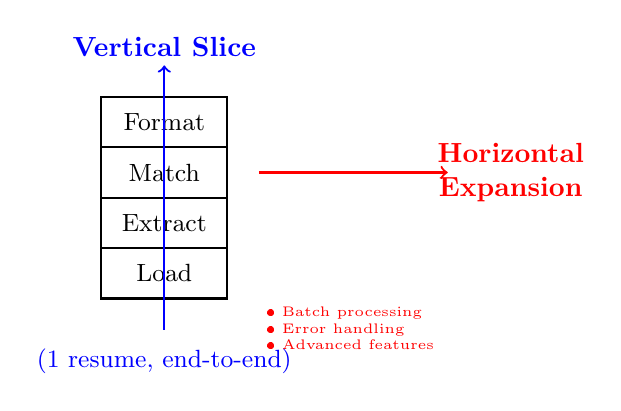
\begin{tikzpicture}[scale=0.8]
    % Vertical slice
    \draw[thick] (0,0) rectangle (2,0.8);
    \draw[thick] (0,0.8) rectangle (2,1.6);
    \draw[thick] (0,1.6) rectangle (2,2.4);
    \draw[thick] (0,2.4) rectangle (2,3.2);

    \node at (1,0.4) {\small Load};
    \node at (1,1.2) {\small Extract};
    \node at (1,2.0) {\small Match};
    \node at (1,2.8) {\small Format};

    \draw[->, thick, blue] (1,-0.5) -- (1,3.7);
    \node[blue] at (1,4) {\textbf{Vertical Slice}};
    \node[blue] at (1,-1) {\small (1 resume, end-to-end)};

    % Horizontal expansion
    \draw[->, thick, red] (2.5,2) -- (5.5,2);
    \node[red, align=center] at (6.5,2) {\textbf{Horizontal}\\\textbf{Expansion}};
    \node[red, align=left, font=\tiny] at (4,-0.5) {
        \begin{tabular}{l}
        • Batch processing\\
        • Error handling\\
        • Advanced features
        \end{tabular}
    };
\end{tikzpicture}
\end{center}
\end{frame}

\begin{frame}{Practical Example: Resume Screening System}
\textbf{Phase 1: Vertical Slice (Crawl)}
\begin{enumerate}
    \item Load one resume text
    \item Call LLM to extract skills
    \item Compare to job requirements
    \item Print result
\end{enumerate}
\vspace{0.3cm}
\textbf{Phase 2: Horizontal Expansion (Walk)}
\begin{itemize}
    \item Process all resumes in a directory
    \item Add structured output (JSON, CSV)
    \item Add confidence scores
    \item Handle missing data gracefully
\end{itemize}
\vspace{0.3cm}
\textbf{Phase 3: Production (Run)}
\begin{itemize}
    \item Optimize prompts and costs
    \item Add caching for repeated skills
    \item Add human-in-the-loop review
    \item Monitor accuracy and performance
\end{itemize}
\end{frame}

\begin{frame}{Design Exercise: Break Into Pieces}
Given the task: \textit{``Build a system to screen IT resumes for a job opening''}
\vspace{0.3cm}

\textbf{What are the system pieces?}
\pause
\begin{enumerate}
    \item \textbf{Input}: Resume PDF/text files, job requirements
    \item \textbf{Parse}: Extract text from PDFs
    \item \textbf{Extract}: Identify skills/technologies from resume
    \item \textbf{Match}: Compare skills to job requirements
    \item \textbf{Score}: Calculate fit score
    \item \textbf{Rank}: Sort candidates by score
    \item \textbf{Output}: Ranked list with justifications
\end{enumerate}
\vspace{0.3cm}
\pause
\textbf{Which piece should we build first?}\\
\pause
$\rightarrow$ The middle pieces (Extract + Match), using sample data!
\end{frame}

\begin{frame}{Key Takeaways: Modular Design}
\begin{enumerate}
    \item \textbf{Break problems into functions with clear inputs/outputs}
    \begin{itemize}
        \item Each function does one thing well
        \item Easy to test, debug, and improve
    \end{itemize}
    \vspace{0.2cm}
    \item \textbf{Build vertical slices first}
    \begin{itemize}
        \item Prove end-to-end flow works with simplest case
        \item Identify integration issues early
    \end{itemize}
    \vspace{0.2cm}
    \item \textbf{Expand horizontally after vertical slice works}
    \begin{itemize}
        \item Add batch processing, error handling, features
        \item Don't optimize or add features prematurely
    \end{itemize}
    \vspace{0.2cm}
    \item \textbf{AI systems benefit especially from this approach}
    \begin{itemize}
        \item LLM behavior is less predictable
        \item Modular design helps isolate and debug issues
        \item Easier to swap models or prompts for specific steps
    \end{itemize}
\end{enumerate}
\end{frame}

\section{Lecture 2: Marketing Automation}

\begin{frame}{What you will build today}
\begin{itemize}
  \item A reproducible workflow that turns lead data into outreach drafts
  \item A quality-control (QC) step that flags risky/low-quality outputs
  \item A simple human-in-the-loop (HITL) review queue for approvals/edits
  \item A tiny evaluation harness to compare prompt versions
\end{itemize}
\end{frame}

\begin{frame}{Business problem}
\textbf{Scenario}: You're on a growth team. You have many inbound leads and limited human time.
\vspace{0.4cm}

\textbf{Goal}: Generate compliant, personalized outreach at scale while minimizing:
\begin{itemize}
  \item hallucinated claims
  \item policy / compliance violations
  \item off-brand tone
  \item missing personalization
\end{itemize}
\end{frame}

\begin{frame}{Inputs (provided in \texttt{lecture\_2/data})}
\begin{itemize}
  \item \texttt{leads.csv}: lead attributes and notes
  \item \texttt{product\_one\_pager.md}: facts you are allowed to use
  \item \texttt{brand\_guidelines.md}: tone and style constraints
  \item \texttt{rubric.md}: what counts as a ``good'' draft
\end{itemize}
\end{frame}

\begin{frame}{Workflow (high-level)}
\begin{enumerate}
  \item \textbf{Summarize} lead notes $\rightarrow$ JSON
  \item \textbf{Draft} email + subject $\rightarrow$ JSON
  \item \textbf{QC} pass: check claims, tone, constraints $\rightarrow$ risk score + reasons
  \item \textbf{HITL} queue: approve / edit / reject
  \item \textbf{Evaluate}: measure pass-rate across a small set
\end{enumerate}
\end{frame}

\begin{frame}{New workflow primitive introduced}
\begin{itemize}
  \item \textbf{Human-in-the-loop review}: you do not ship raw model output to customers
  \item \textbf{Evaluation harness}: treat prompt edits like code changes (measure impact)
\end{itemize}
\end{frame}

\begin{frame}{Structured output schemas (examples)}
\textbf{Lead summary schema}
\begin{itemize}
  \item \texttt{lead\_summary} (string)
  \item \texttt{pain\_points} (list[string])
  \item \texttt{suggested\_angle} (string)
  \item \texttt{missing\_info} (list[string])
\end{itemize}
\vspace{0.3cm}
\textbf{Draft schema}
\begin{itemize}
  \item \texttt{subject} (string)
  \item \texttt{email\_body} (string)
  \item \texttt{personalization\_tokens} (list[string])
\end{itemize}
\end{frame}

\begin{frame}{Exercises}
\begin{itemize}
  \item Baseline prompt $\rightarrow$ get working JSON output
  \item Improve personalization while keeping compliance constraints
  \item Add QC checks: hallucination/claims, tone, forbidden phrases
  \item Implement a HITL review loop in the notebook
  \item Run the mini-eval and compare prompt versions
\end{itemize}
\end{frame}

\begin{frame}{Deliverable}
\begin{itemize}
  \item \texttt{notebooks/lecture\_2\_marketing\_hitl.ipynb}
  \item Output files in \texttt{data/outputs/}:
    \begin{itemize}
      \item \texttt{drafts.csv} (final approved drafts)
      \item \texttt{qc\_report.csv} (scores + reasons)
    \end{itemize}
\end{itemize}
\end{frame}

\begin{frame}{Extensions / Optional challenges}
\begin{itemize}
  \item \textbf{Rubric-based grader}: have the model score drafts using \texttt{rubric.md}; compare to human scores
  \item \textbf{Batching + cost controls}: cache summaries; estimate tokens/cost; compare one-pass vs two-pass QC
  \item \textbf{Policy-driven compliance}: map \texttt{compliance\_tags} to explicit deny/allow rules and required disclaimers
  \item \textbf{Prompt/version tracking}: log prompts + model + params alongside outputs for reproducibility
  \item \textbf{Multi-variant testing}: A/B prompt variants; select winners by eval metrics
\end{itemize}
\end{frame}

\begin{frame}{Discussion}
\begin{itemize}
  \item Where did the model fail? (missing facts vs wrong facts vs style)
  \item What did structured output enable?
  \item What checks should be automated vs left to humans?
  \item How do cost and latency constrain the pipeline?
\end{itemize}
\end{frame}

\begin{frame}{Next time}
\begin{itemize}
  \item Add external actions (APIs) and state management
  \item Ground responses in a knowledge base
\end{itemize}
\end{frame}

\end{document}

